\documentclass[11pt]{beamer}
%\documentclass[11pt,handout]{beamer}

\usepackage{multimedia}

%\usetheme[secheader]{Boadilla}
\usetheme{Boadilla}

%\setbeameroption{hide notes}
%\setbeameroption{show notes}
%\setbeameroption{show only notes}
%\setbeamertemplate{note page}[plain]

\usefonttheme{structuresmallcapsserif}
\setbeamerfont{frametitle}{size=\normalsize}
\setbeamertemplate{navigation symbols}{}

\AtBeginSection[]{}

\setbeamercovered{invisible}

% Customization
%\usepackage{bibentry}
%\newcommand{\footcite}[1]{$^[$\footnote{\begin{tiny}\bibentry{#1}\end{tiny}}$^]$}
\usepackage[natbib=true, bibstyle=numeric, citestyle=authoryear,
            uniquename=false, uniquelist=false,
            firstinits=true, maxcitenames=3, minbibnames=3, maxbibnames=4,
            dashed=false, url=false, doi=false, isbn=false]{biblatex}
\newrobustcmd*{\citepub}{%
  \AtNextCite{\defcounter{minnames}{4}}\fullcite}
\newcommand{\footcitefull}[1]{$^[$\footnote{\begin{tiny}\citepub{#1}\end{tiny}}$^]$}
\addbibresource{../literature.bib}

\renewcommand{\emph}[1]{\textbf{#1}}

% Author, Title, etc.
\title[BayesOpt 2015]{Active Contextual Entropy Search}
\author[Jan Hendrik Metzen]{Jan Hendrik Metzen}
\institute[]{AG Robotik, University Bremen\\ Project BesMan \url{http://robotik.dfki-bremen.de/en/research/projects/besman.html}}
\date[12/12/15]{BayesOpt 2015, December 12, 2015}

\begin{document}

\frame{\titlepage}

\begin{frame}{Overview}
   \begin{itemize}
     \item We apply Bayesian optimization to multi-task robotic behavior learning  (contextual policy search\footcitefull{deisenroth_survey_2013})
     \item We focus on problems
     \begin{itemize}
       \item which are low-dimensional
       \item where the possible number of evaluations is very small
       \item thus, in general, well-suited for Bayesian optimization\footcitefull{metzen_bayesian_2015}
     \end{itemize}
     \item We propose \emph{Active Contextual Entropy Search} (ACES)
     \begin{itemize}
       \item an extension of entropy search\footcitefull{hennig_entropy_2012}
       \item suited for contextual problems (multi-task learning)
       \item allows actively selecting contexts (active learning)
     \end{itemize}
   \end{itemize}
\end{frame}

\begin{frame}{Results}
   \begin{itemize}
     \item \emph{Scenario:} Simulated ball-throwing with a robotic arm
    \end{itemize}
    \begin{center}
       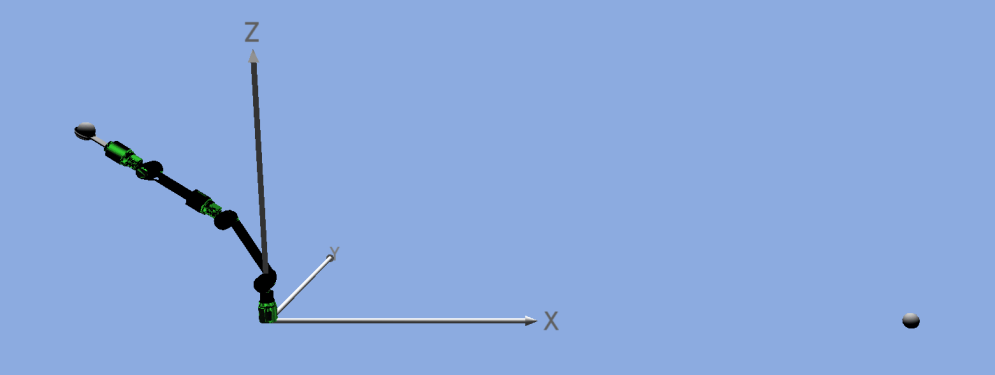
\includegraphics[width=.4\textwidth]{pics/compi.png}
       \hspace{1cm}
       \includegraphics[width=.25\textwidth]{pics/xy_scatter_color_g0}
   \end{center}

   \vspace*{-.5cm}
   \begin{center}
       \begin{minipage}[b][5cm][c]{.59\textwidth}
        \begin{itemize}
            \item To be learned: generalization of throw behavior to different target positions (contexts)
            \item Movement primitive fixed, only meta-parameters adapted
            \item ACES allows actively selecting target positions to be practiced
            \item ACES outperforms passive task selection
        \end{itemize}
        \end{minipage}
       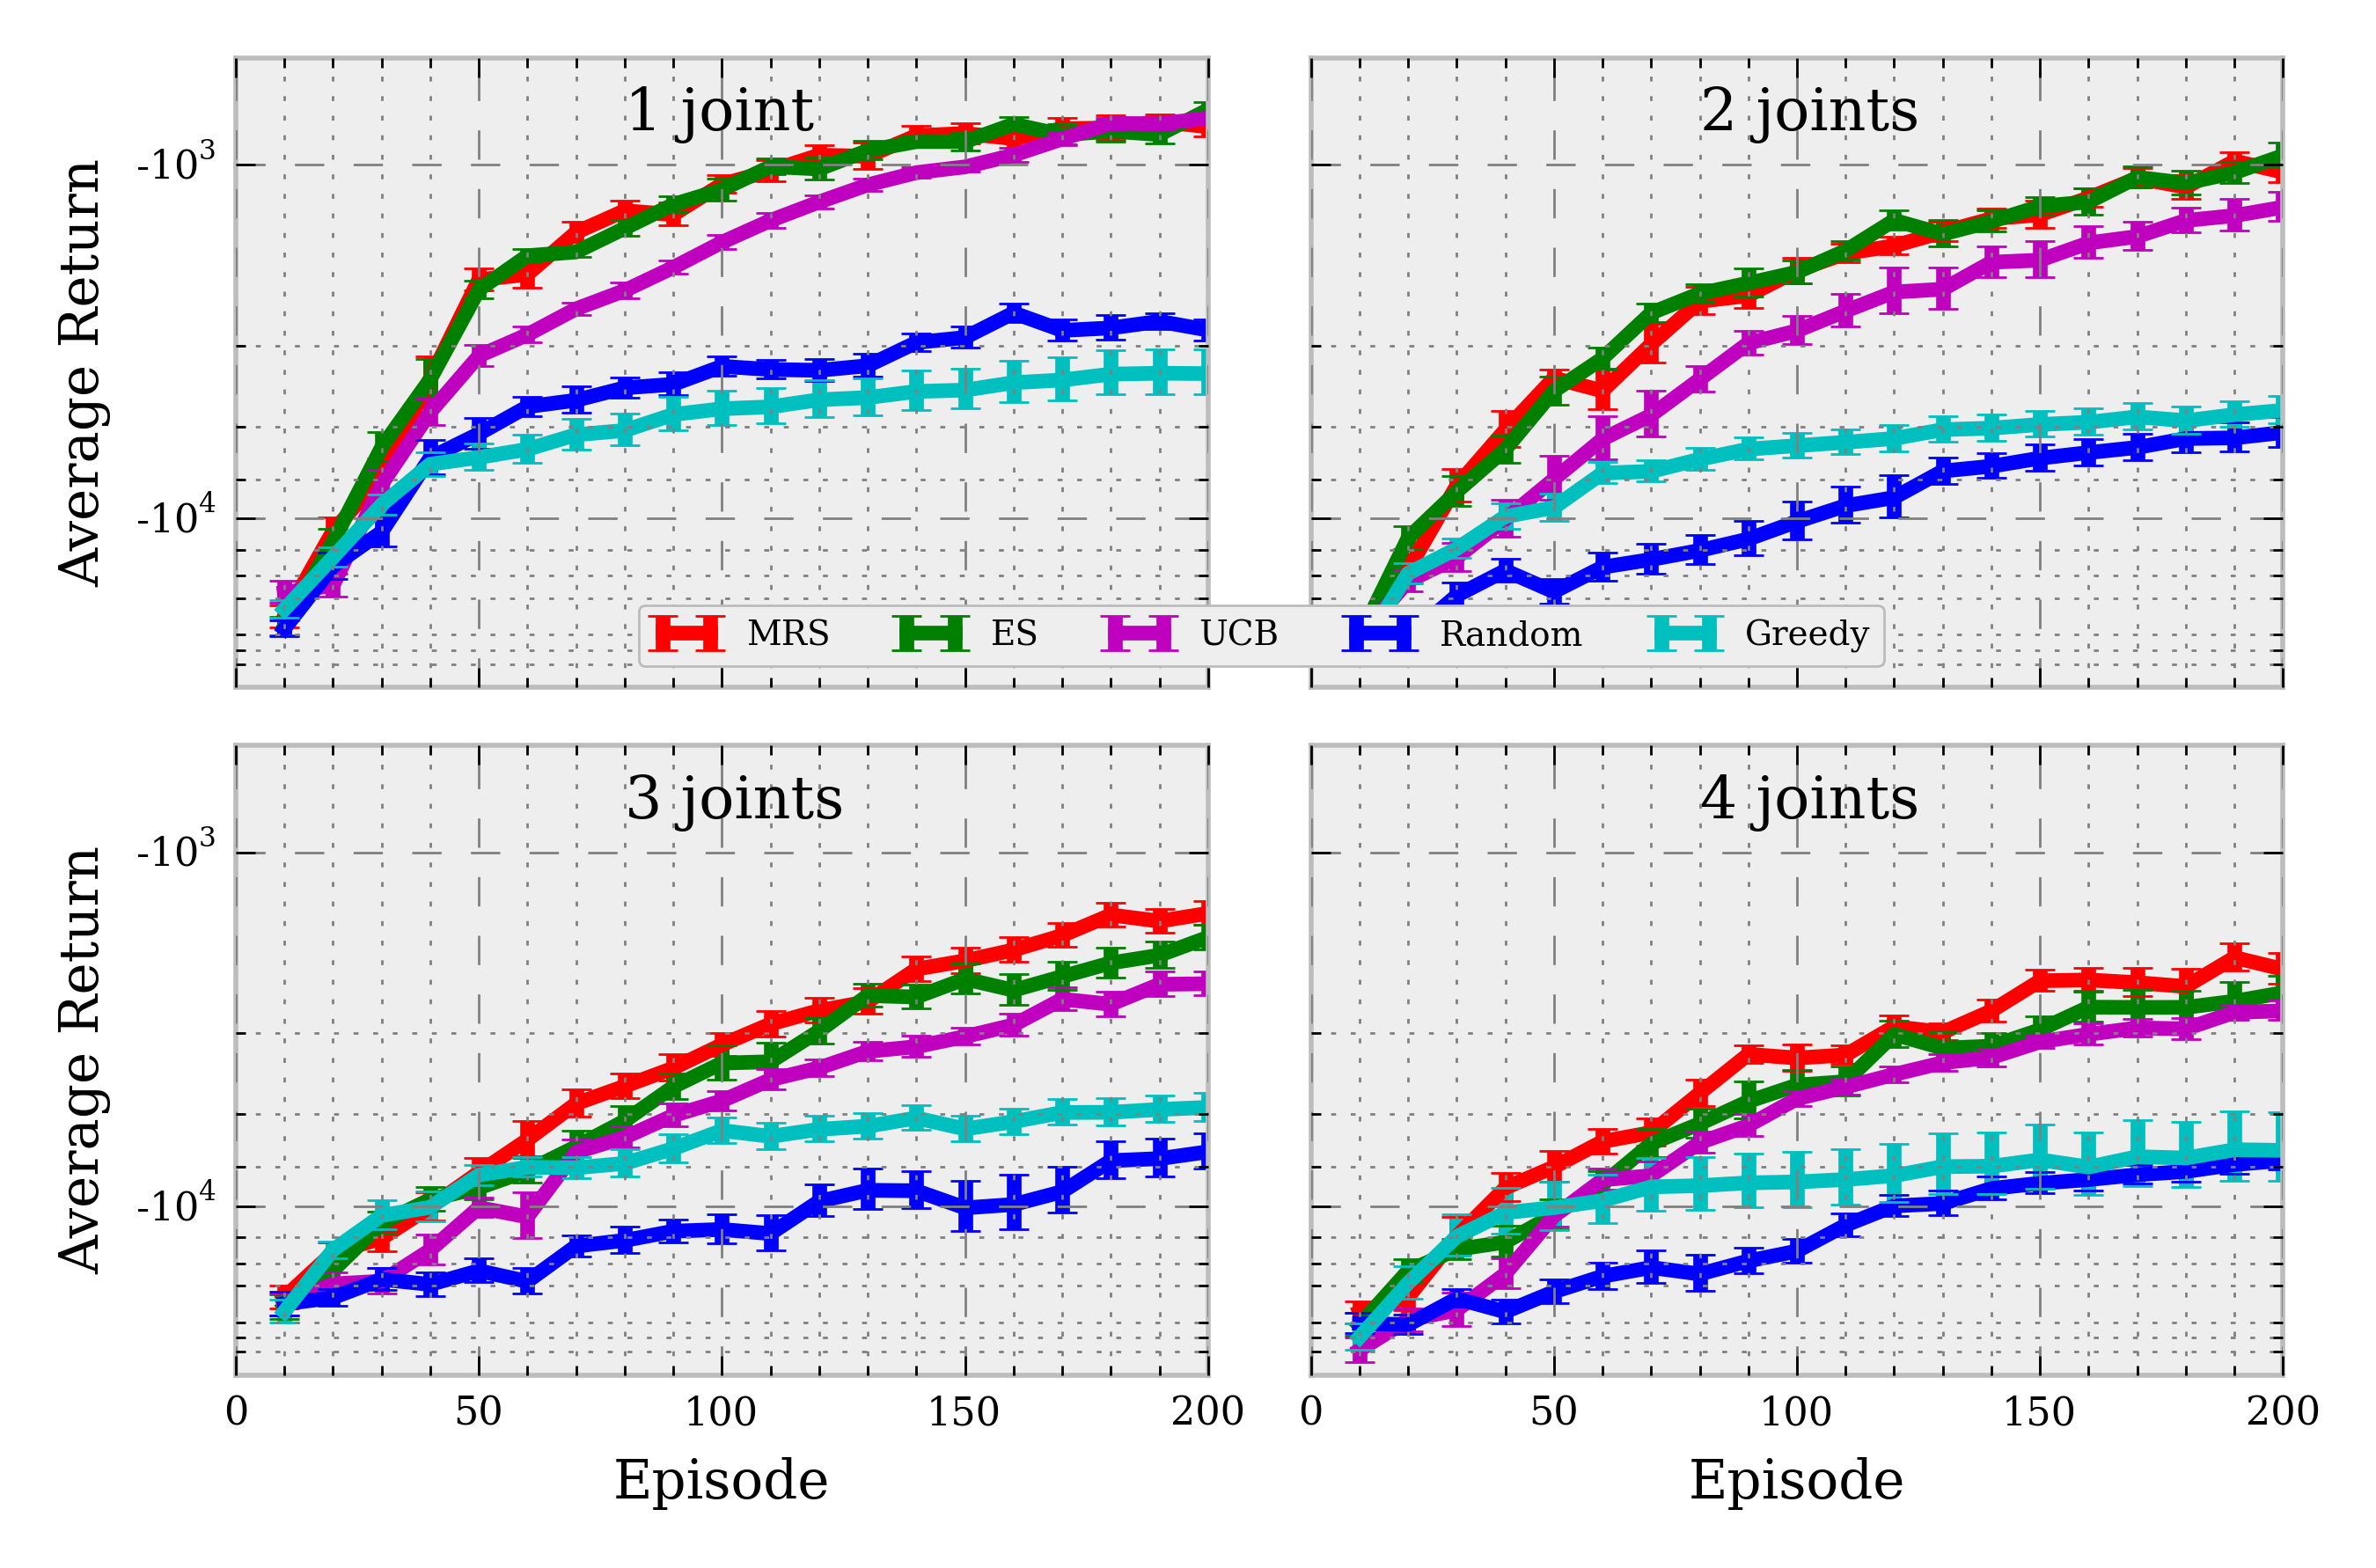
\includegraphics[width=.4\textwidth]{../pics/learning_curve}
   \end{center}
   \vspace*{-.5cm}
   \begin{center}
   More details on the poster. Hope to see you there!
   \end{center}
\end{frame}
\end{document}
